The purpose of this algorithm is tracking objects, producing added informations about the followed target.
The algorithm developed takes as inputs sequential frames and Region Of Interesting(ROI). They are important to
define the parameters used to generate the tracking of objects and other details as: the relative velocity, the factor of 
approaching and of departure

With ROI determined, the system enters in looping to follow the target as shown in the fig. 1.

\begin{figure}[bhp]
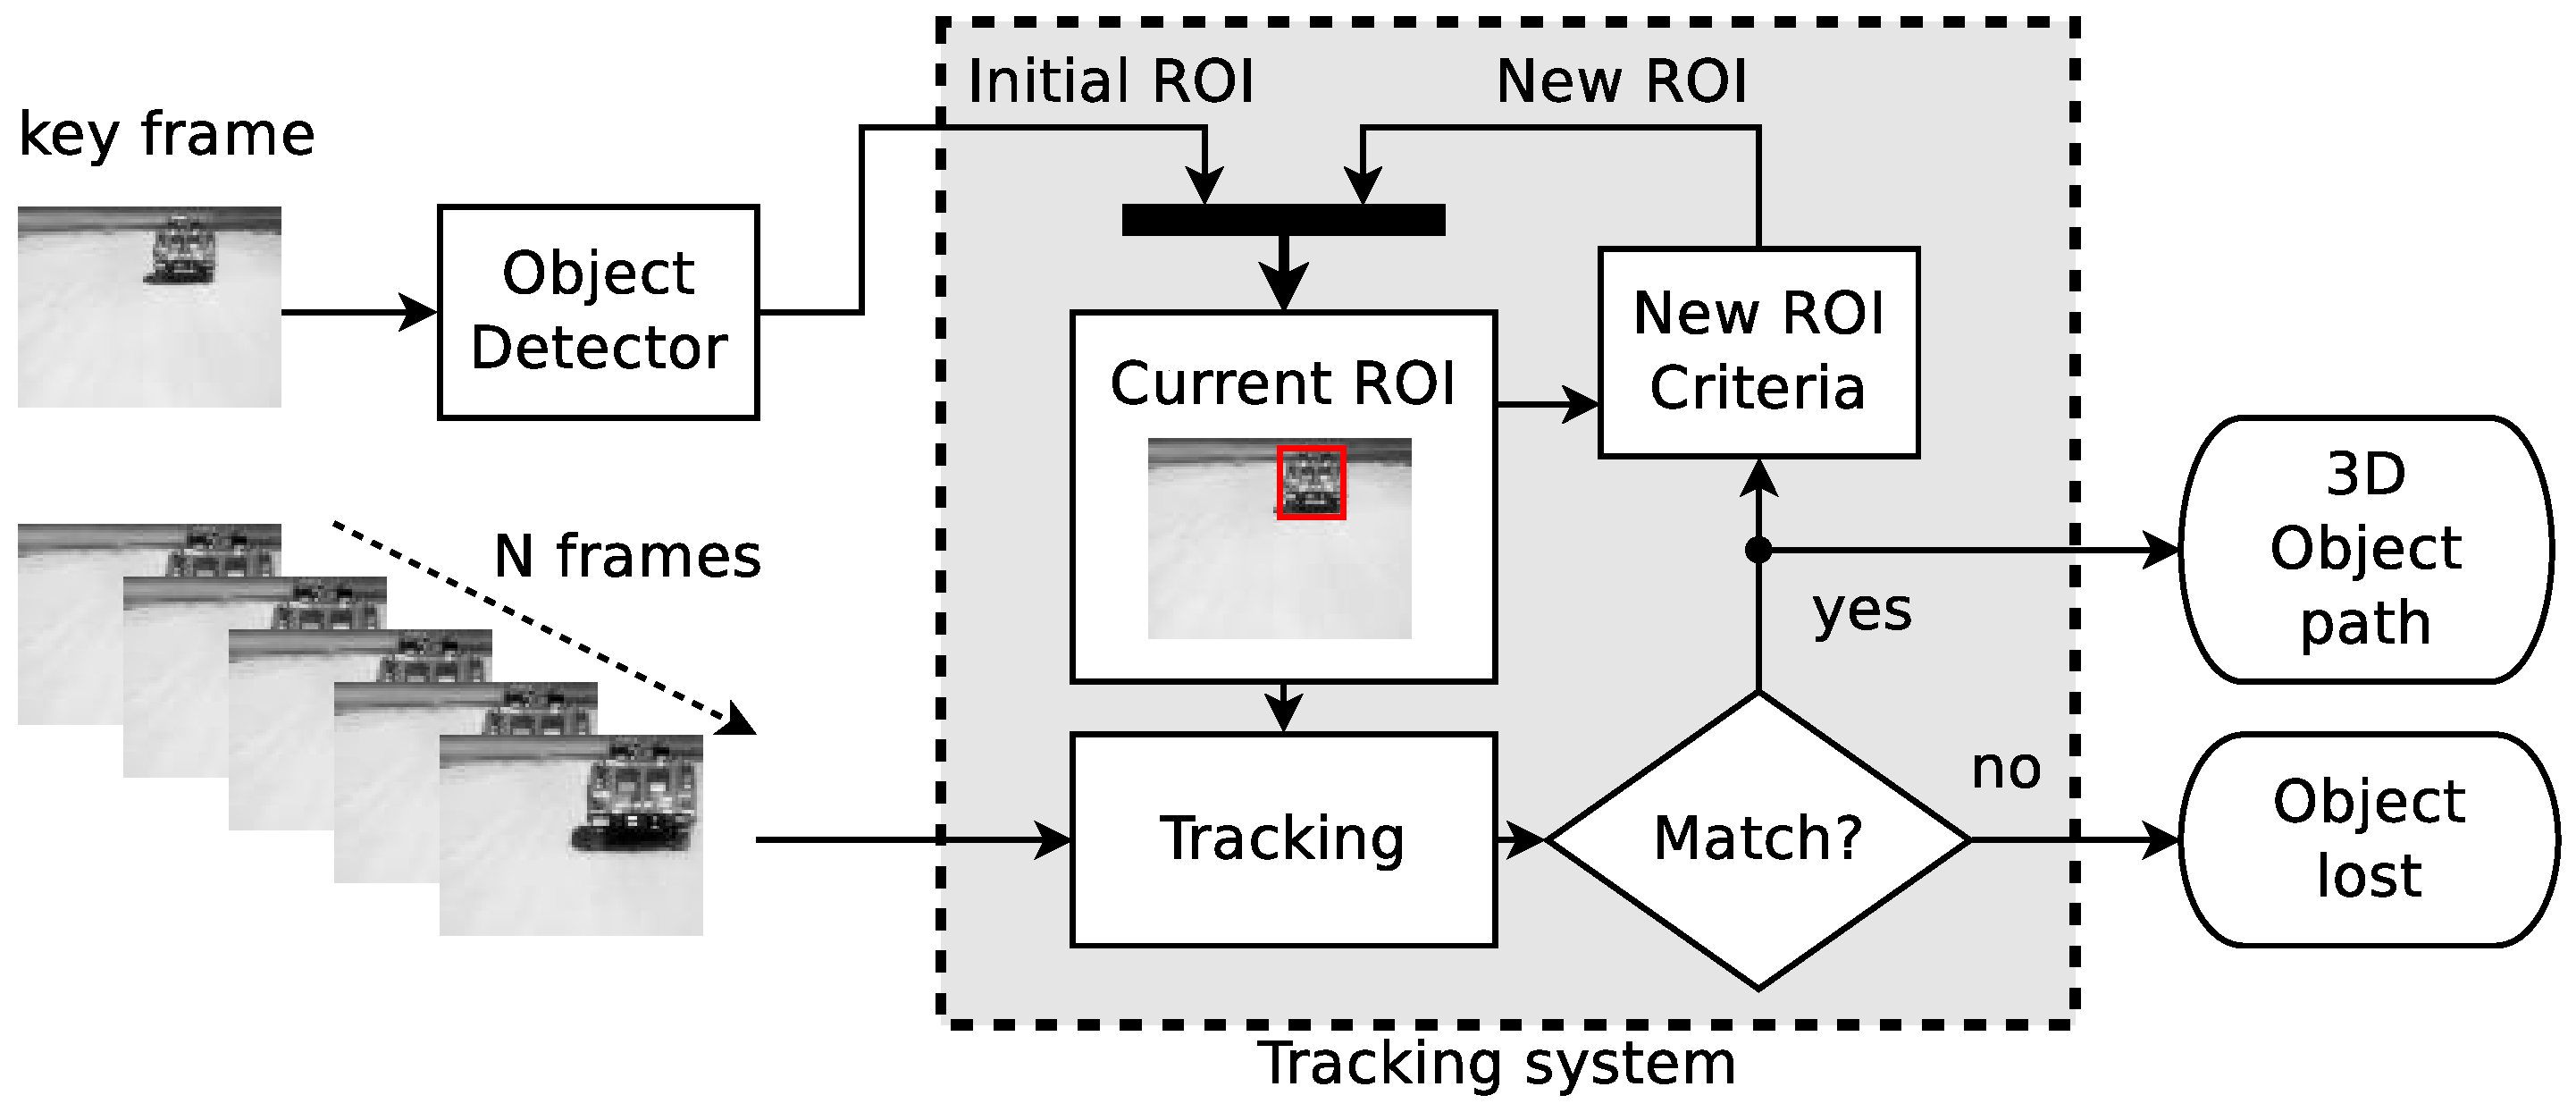
\includegraphics[width=\columnwidth]{images/figure1-diagram1.eps}
\caption{With object detected, the highest value of PCC in the Window Of Search (WOS) of next frame identifies the target, 
and the result of search is a vector. 
Which its beginning and its end are on the first and last position, respectively. After, these processing is made again for 
next frames.}
\end{figure}

In 2 dimensions, the objects are tracking and given information about its horizontal or vertical relative velocity.
When the target moves in 3 dimensions, outputs are the resultant of relative velocity and the factor of approaching or departure. 
There isn't a factor in 2 dimensions, since approaching or departure don't exist in this situation.

%Diagrama1
 %A gente vai explicar o algoritmo como uma caixa fechada , que coisa entra e que coisa sai
 %e os parametros a sintonizar.
 % como usar ele quando implementado, como se fosse uma caixa preta.
